\documentclass[11pt]{article}
\usepackage[margin=1in]{geometry}
\usepackage{amsmath,amssymb}
\usepackage{tikz}
\usepackage{float}
\usepackage{graphicx}
\usepackage[hidelinks]{hyperref}

\setlength{\parindent}{0pt}
\setlength{\parskip}{0.7\baselineskip}

\begin{document}

\section{Global Constraints}

We've seen at least one of these in action: all-different -- now we will talk about them in a bit more.

Global constraints allow expressing a constraint between a non-fixed number of variables.

\textbf{Global constraints} have many advantages, including that they:
\begin{itemize}
    \item let us express constraints that occur in our models more compactly and intuitively;
    \item may come with special algorithms to compute them more efficiently;
    \item may allow for better inference/propagation (beyond basic arc consistency).
\end{itemize}

The plan:
\begin{itemize}
    \item look at all-different
    \begin{itemize}
        \item increased expressiveness
        \item matching-based algorithm
    \end{itemize}
    \item look at the circuit constraint
    \begin{itemize}
        \item sub-tour elimination via a union-find-based chain rule
    \end{itemize}
    \item (maybe) look at other global constraints via the \href{http://www.dcs.gla.ac.uk/~pat/cpM/minizincCPM/tutorial/minizinc-tute.pdf}{MiniZinc catalogue and tutorial}
    \begin{itemize}
        \item cardinality constraint
    \end{itemize}
\end{itemize}

\subsection{All-different}

Remember our requirement from assignment 1 that all arrivals must be on different days? At least one possible solution used all-different.

$n$-Queens is a classic problem used to introduce all-different (and a fun problem!) so we'll discuss it.

\begin{figure}[H]
    \centering
    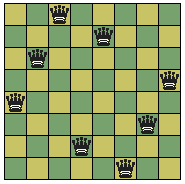
\includegraphics[width=0.35\textwidth]{image.png}
    \caption{Eight queens. \emph{(User:Lee Daniel Crocker -- modified by Fispaul at da.wikipedia, CC BY-SA 3.0, via Wikimedia Commons.)}}
\end{figure}

\begin{description}
    \item[Instance:] a natural number $n$;
    \item[Question:] can we place $n$ queens on an $n \times n$ chessboard so that no two are in the same row, column, or diagonal?
\end{description}

Expressing this without all-different is possible but annoying. With all-different it is straightforward in MiniZinc:

(we'll look at an example board in lecture to make sure we understand encoding)

\begin{verbatim}
int: n;
array [1..n] of var 1..n: X;
include "alldifferent.mzn";
%distinct columns
constraint alldifferent(X);
 % distinct diagonals upwards
constraint alldifferent([ X[i] + i - 1| i in 1..n]);
 % distinct diagonals downwards
constraint alldifferent([ X[i] - i + 1| i in 1..n]);

solve satisfy;
\end{verbatim}

Partial search tree from the \href{http://www.dcs.gla.ac.uk/~pat/cpM/minizincCPM/tutorial/minizinc-tute.pdf}{MiniZinc tutorial}:

\begin{figure}[H]
    \centering
    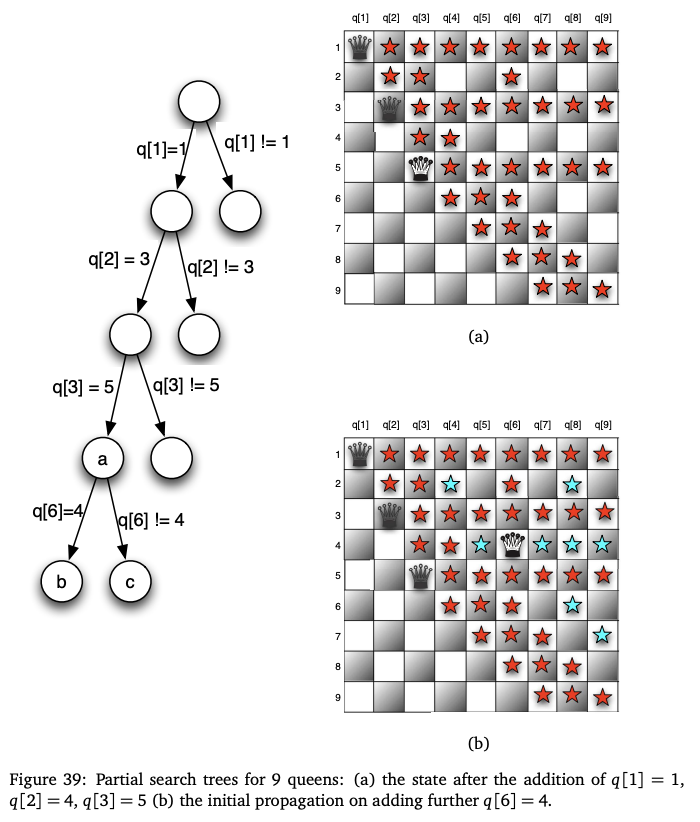
\includegraphics[width=0.85\textwidth]{image-1.png}
    \caption{Partial search tree for the $n$-queens problem.}
\end{figure}

So hopefully I've convinced you that it's convenient for encoding. Let's talk inference (in a smaller pseudo-code example):

\[
    x, y, z \in \mathbb{N}, \qquad D(x) = D(y) = \{1, 2\}, \qquad D(z) = \{1, 2, 3\}, \qquad \text{all-different}(x, y, z)
\]

What can we infer about $z$? Could we get this from arc consistency if we just had $x\neq y$, $x \neq z$, $y \neq z$ as our constraints?

This sort of thing might be familiar to anyone who does sudoku puzzles, and is a powerful thing about all-different.

\subsection{Matchings for all-different}

We want to exclude domain values that are not part of any all-different value assignment. Luckily, graph theory can help us with \textbf{maximum matchings}.

Let's visualise our possible assignments as a bipartite graph (that is, a graph with two parts that only has edges between the parts):
\begin{itemize}
    \item the vertex set of one part is the variables that are all-different;
    \item the vertex set of the other part is the possible values;
    \item there is an edge from variable $v$ to value $d$ if $d$ is in $D(v)$.
\end{itemize}

(We will draw this out for our small example above.)

A maximum matching on a bipartite graph like this is a set of edges such that:
\begin{itemize}
    \item no two edges share an endpoint;
    \item there are as many edges in this set as possible.
\end{itemize}

If our problem is satisfiable, then there must be a matching that is as large as the set of all-different variables.

\textbf{Proof sketch}, where $V_1$ is the set of variables and $V_2$ is the set of values:
\begin{itemize}
    \item \emph{Satisfiable implies matching.} Take the satisfying assignment $\Phi: V_1 \rightarrow V_2$. As it is satisfying, we know that $|\Phi| = |V_1|$ and $\Phi(v_i) \neq \Phi(v_j)$ for all distinct $v_i, v_j \in V_1$. Then take the set of edges $E_M = \{(v, x)\}$ where $v \in V_1$, $x \in V_2$, and $\Phi(v) = x$. We still need to show that:
    \begin{itemize}
        \item $|E_M| = |V_1|$;
        \item $E_M$ are edges in our graph;
        \item for every pair of edges $(v, x)$ and $(u, z)$ in $E_M$ we have that $v \neq u$ and $x \neq z$.
    \end{itemize}
    \item Let's do the second part together in lecture.
\end{itemize}

Alright, so we're only interested in edges that are in \emph{some} max matching, but how can we tell that?

Jack Edmonds and Claude Berge can help:

\begin{figure}[H]
    \centering
    
\includegraphics[width=0.4\textwidth]{image-2.png}\hfill
    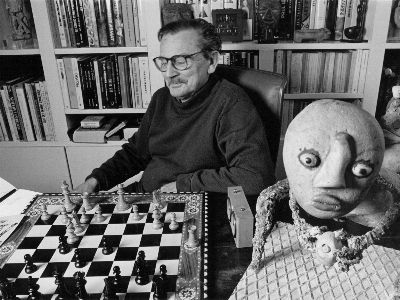
\includegraphics[width=0.4\textwidth]{image-3.png}
    \caption{Jack Edmonds and Claude Berge.}
\end{figure}

(Claim due to Berge, algorithm from Edmonds.)

\begin{quote}
An edge belongs to some but not all maximum matchings if and only if, for an arbitrary maximum matching, it belongs to either an even alternating path which begins at a free node, or an even alternating cycle.
\end{quote}

OK, we've been lazy. Some definitions. Let $M$ be a matching.
\begin{itemize}
    \item An edge in $M$ is a \emph{matching edge}; every edge not in $M$ is \emph{free}.
    \item A node is \emph{matched} if it is incident to a matching edge, and \emph{free} otherwise.
    \item An \emph{alternating path} or \emph{cycle} is a path or cycle whose edges are alternately matching and free.
\end{itemize}

We'll draw a picture in lecture -- possibly a little one and a big one.

What complexity is this? Note that you couldn't really work it out without specifying our alternating path algorithm -- we'll just state it here to consider how fast it is compared with a full search tree.

If we are enforcing all-different over $k$ variables, and the largest domain over those variables is size $m$, then $O(km\sqrt{k})$ to get matchings information, which dominates.

The main thing to notice is that this is much faster than a full search, so likely saves us time.

A few resources:
{\small
\begin{itemize}
    \item \url{https://www.cs.upc.edu/~erodri/webpage/cps//theory/cp/global-constraints/slides.pdf}
    \item \url{https://www.sciencedirect.com/science/article/pii/S1574652606800106}
    \item \url{http://www.constraint-programming.com/people/regin/papers/globalCpaior.pdf}
\end{itemize}
}

\subsection{Circuit constraint}

We've just seen all-different, filtered to full arc consistency via maximum bipartite matching. Now consider a second global constraint, \texttt{circuit}, together with a filtering technique for it based on a union-find structure.

\subsubsection{Definition}

Fix $n \in \mathbb{N}$ and index a set of $n$ objects (cities, tasks, locations) by $\{1,\dots,n\}$. Introduce one variable per index,
\[
    \text{succ}[i] \in \{1,\dots,n\}, \qquad i = 1,\dots,n,
\]
with the intended meaning that object $i$ is followed by object $\text{succ}[i]$.

The constraint $\texttt{circuit}(\text{succ})$ holds exactly when $\text{succ}$, viewed as a function $\{1,\dots,n\}\to\{1,\dots,n\}$, is a single $n$-cycle: $\text{succ}$ is a fixed-point-free permutation of $\{1,\dots,n\}$, and iterating $\text{succ}$ from any index visits all $n$ indices before returning to it.

This is the natural model for a travelling-salesperson-style problem: assign every location a successor, then (in the optimisation version) minimise total edge cost.

\subsubsection{All-different is necessary but not sufficient}

$\text{succ}$ must certainly be all-different: no two indices can share a successor, and no index can be its own successor. But a fixed-point-free permutation need not be a single cycle -- it can decompose into several disjoint cycles.

\textbf{Example.} Take $n = 4$ and $\text{succ} = [2, 1, 4, 3]$. This is a fixed-point-free permutation, so all-different is satisfied, yet
\[
    1 \to 2 \to 1 \qquad \text{and} \qquad 3 \to 4 \to 3
\]
are two disjoint $2$-cycles rather than one $4$-cycle (Figure~\ref{fig:subtour}).

\begin{figure}[H]
    \centering
    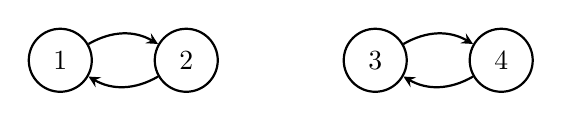
\begin{tikzpicture}[
        every node/.style={circle,draw,fill=white,minimum size=8mm,inner sep=0pt},
        ->,>=stealth,thick
    ]
        \node (n1) at (0,0) {1};
        \node (n2) at (1.6,0) {2};
        \node (n3) at (4,0) {3};
        \node (n4) at (5.6,0) {4};

        \draw (n1) to[bend left=30] (n2);
        \draw (n2) to[bend left=30] (n1);
        \draw (n3) to[bend left=30] (n4);
        \draw (n4) to[bend left=30] (n3);
    \end{tikzpicture}
    \caption{$\text{succ}=[2,1,4,3]$: all-different holds, but the result is two disjoint 2-cycles, not a single circuit.}
    \label{fig:subtour}
\end{figure}

All-different filtering therefore cannot rule out sub-tours; an additional propagation rule is required.

\subsubsection{Chains and a pruning rule}

Suppose a subset of the $\text{succ}$ variables has been fixed. The fixed edges $(i,\text{succ}[i])$ decompose into disjoint directed paths, or \emph{chains}; an index whose variable is not yet fixed forms a chain of length one on its own.

For an index $x$ lying on some chain, write $\text{start}(x)$ for the first index of that chain and $\text{end}(x)$ for the last, and let $\text{len}(x)$ be the number of indices on the chain. Fixing $\text{succ}[i]=j$ merges the chain ending at $i$ with the chain starting at $j$; the merged chain runs from $\text{start}(i)$ to $\text{end}(j)$, with length $\text{len}(i)+\text{len}(j)$.

\textbf{Pruning rule.} If $x$ lies on a chain with $\text{start}(x)=s$, $\text{end}(x)=e$, and $\text{len}(x) < n$, remove $s$ from $D(\text{succ}[e])$: setting $\text{succ}[e]=s$ would close a cycle of length $\text{len}(x) < n$, a sub-tour. Once $\text{len}(x)=n$, the edge $\text{succ}[e]=s$ closes the unique Hamiltonian circuit and must not be pruned.

Maintaining $\text{start}$, $\text{end}$, and $\text{len}$ under repeated merges is exactly what a \textbf{union-find} (disjoint-set) structure with path compression provides, in amortised time $O(\alpha(n))$ per operation, where $\alpha$ is the inverse Ackermann function.

This is essentially the \texttt{nocycle} propagator of Caseau and Laburthe (1997); see the resources below.

\subsubsection{Worked example}

Take $n=5$ and fix $\text{succ}[1]=3$, then $\text{succ}[3]=5$, then $\text{succ}[5]=2$, in that order. Two filters act throughout: the pruning rule above, and all-different (an already-claimed successor value cannot be reused elsewhere).

Initially $D(\text{succ}[i]) = \{1,\dots,5\}\setminus\{i\}$ for every $i$.

\begin{itemize}
    \item $\text{succ}[1]=3$: chain $1\to 3$, length $2$. Pruning rule removes $1$ from $D(\text{succ}[3])$, giving $D(\text{succ}[3])=\{2,4,5\}$.
    \item $\text{succ}[3]=5$: chain $1\to3\to5$, length $3$. Pruning rule removes $1$ from $D(\text{succ}[5])$, giving $D(\text{succ}[5])=\{2,3,4\}$.
    \item $\text{succ}[5]=2$: chain $1\to3\to5\to2$, length $4$. Pruning rule removes $1$ from $D(\text{succ}[2])$.
\end{itemize}

\begin{figure}[H]
    \centering
    \begin{tikzpicture}[
        every node/.style={circle,draw,fill=white,minimum size=8mm,inner sep=0pt},
        ->,>=stealth,thick
    ]
        \node (n1) at (0,0) {1};
        \node (n3) at (2,0) {3};
        \node (n5) at (4,0) {5};
        \node (n2) at (6,0) {2};
        \node (n4) at (3,1.8) {4};

        \draw (n1) -- (n3);
        \draw (n3) -- (n5);
        \draw (n5) -- (n2);
        \draw[dashed] (n2) to[out=250,in=290,looseness=1.8] (n1);
        \node[draw=none,fill=none] at (3,-2.9) {\footnotesize pruned};
    \end{tikzpicture}
    \caption{State after fixing $\text{succ}[1]=3$, $\text{succ}[3]=5$, $\text{succ}[5]=2$: a single chain $1\to3\to5\to2$ of length $4<5$, index $4$ still unattached, and the closing edge $\text{succ}[2]=1$ pruned.}
    \label{fig:partial-chain}
\end{figure}

At this point $D(\text{succ}[2]) = \{1,3,4,5\}\setminus\{1,3,5\} = \{4\}$: $3$ and $5$ are removed by all-different (already claimed by $1$ and $3$ respectively), and $1$ by the pruning rule. So $\text{succ}[2]=4$ is forced.

This extends the chain to $1\to3\to5\to2\to4$, length $5=n$. Now $D(\text{succ}[4]) = \{1,2,3,5\}\setminus\{2,3,5\}=\{1\}$, and since $\text{len}=n$ the pruning rule permits $\text{succ}[4]=1$.

\begin{figure}[H]
    \centering
    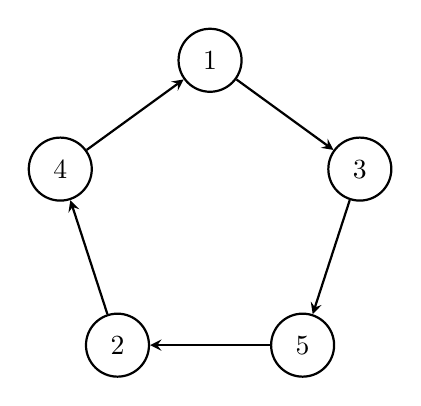
\begin{tikzpicture}[
        every node/.style={circle,draw,fill=white,minimum size=8mm,inner sep=0pt},
        ->,>=stealth,thick
    ]
        \node (a) at (90:2) {1};
        \node (b) at (18:2) {3};
        \node (c) at (-54:2) {5};
        \node (d) at (-126:2) {2};
        \node (e) at (-198:2) {4};

        \draw (a) -- (b);
        \draw (b) -- (c);
        \draw (c) -- (d);
        \draw (d) -- (e);
        \draw (e) -- (a);
    \end{tikzpicture}
    \caption{The completed circuit $1\to3\to5\to2\to4\to1$.}
    \label{fig:full-circuit}
\end{figure}

Propagation alone determines the full circuit from three initial decisions, with no search.

\subsubsection{Completeness}

Union-find keeps this filtering cheap: $O(n\,\alpha(n))$ overall. It is not, however, complete. Full generalised arc consistency for \texttt{circuit} would require deciding, for every remaining candidate value of every variable, whether it extends to some Hamiltonian circuit consistent with the current domains. Taking domains directly from a graph's adjacency structure reduces this decision problem to deciding Hamiltonicity of that graph, which is NP-complete (Karp, 1972). So no polynomial-time filtering algorithm achieves full consistency for \texttt{circuit} unless $P=NP$. The pruning rule above is sound but incomplete, and is used together with all-different's matching-based filter, which is complete for all-different on its own.

\subsubsection{Circuit in MiniZinc}

\begin{verbatim}
int: n;
array[1..n] of var 1..n: succ;
include "circuit.mzn";
constraint circuit(succ);

solve satisfy;
\end{verbatim}

The all-different filtering, chain tracking, and sub-tour pruning above all take place inside this single \texttt{circuit(succ)} call.

The optimisation version (shortest tour, i.e.\ classic TSP) adds costs and an objective:

\begin{verbatim}
int: n;
array[1..n, 1..n] of int: cost;
array[1..n] of var 1..n: succ;
include "circuit.mzn";
constraint circuit(succ);

solve minimize sum(i in 1..n)(cost[i, succ[i]]);
\end{verbatim}

A few resources:
{\small
\begin{itemize}
    \item Y.\ Caseau and F.\ Laburthe, ``Solving Small TSPs with Constraints,'' \emph{Proc.\ 14th International Conference on Logic Programming (ICLP)}, MIT Press, 1997, pp.\ 316--330. Available at \url{https://www.dcs.gla.ac.uk/~pat/cpM/papers/caseau97solving.pdf}
    \item R.\ M.\ Karp, ``Reducibility Among Combinatorial Problems,'' in \emph{Complexity of Computer Computations}, Plenum Press, 1972, pp.\ 85--103.
    \item \url{https://www.minizinc.org/doc-2.3.0/en/lib-globals.html} (see \texttt{circuit})
\end{itemize}
}

\subsection{Global cardinality constraint}

This is a generalisation of the all-different constraint:
\begin{itemize}
    \item a set of variables $X$ take their values from domain $D$, and the constraint restricts the number of times that any value can be assigned to variables, within some range.
\end{itemize}

Example: remember rota scheduling? We might have some minimum and maximum possible number of people working each night/day shift. Of course we can do this without a global constraint, but it makes it easier (and faster!) as with all-different.

Pulling a code snippet out for the guards rota example (full examples and problem description at \url{https://github.com/magicicada/cp/tree/main/week_by_week/week_3/afternoon_examples/guard_rota}):

Without global cardinality:
\footnotesize
\begin{verbatim}
% the number of guards that must be on duty in each shift of each day
array[DAYS] of var lwbDay .. upbDay: totalOnDay;
constraint forall(d in DAYS)(
    totalOnDay[d] = sum(g in GUARDS)(roster[g,d] = DAY));
array[DAYS] of var lwbNight .. upbNight: totalOnNight;
constraint forall(d in DAYS)(
    totalOnNight[d] = sum(g in GUARDS)(roster[g,d] = NGT));
\end{verbatim}
\normalsize

With:
\footnotesize
\begin{verbatim}
% the number of guards that must be on duty in each shift of each day
array[DAYS] of var lwbDay..upbDay: totalOnDay;
array[DAYS] of var lwbNight..upbNight: totalOnNight;
constraint forall(d in DAYS)(
    global_cardinality([roster[g,d] | g in GUARDS],
        [DAY,NGT],[totalOnDay[d],totalOnNight[d]]));
\end{verbatim}
\normalsize

\subsection{Summary}

As a general message: these special global constraints are expressive, and typically faster than rolling your own. Some, like all-different, admit filtering that is both cheap and complete; others, like circuit, only admit filtering that is cheap but incomplete (full consistency for circuit is NP-hard) -- still very much worth having, just not the whole story on their own.

Try to use them when you can! See the \href{https://www.minizinc.org/doc-2.3.0/en/lib-globals.html}{MiniZinc global constraints library}.

\end{document}
